\refstepcounter{section}
\section*{Lecture 08: Mean-field solution for Ising model}
\addcontentsline{toc}{section}{Lecture 08: Mean-field solution for Ising model}
We will continue our discussion of the mean-field solution of the Ising model. Previously, we had reduced the Hamiltonian to a simplified expression, with an effective field. 
$$\SH =  -\mathrm{h}_{\text{\tiny eff}} \sum_i \sigma_i +\frac{JN\gamma}{2}\avg{\sigma}^2$$
This is simple to solve, since this is $N$ independent spins in a field. The partition function is, 
\begin{align}
    \SZ = \sum_{\{\sigma_i\}} e^{\beta \mathrm{h}_{\text{\tiny eff}}\sum \sigma_i} \cdot e^{-\beta\SE\tund{0}}
\end{align} 
where $\SE\tund{0} = \frac{J\gamma N}{2}\avg{\sigma}^2$. Since the particles are independent, the sum over spins can be simplified as,
$$\SZ = \qty[\sum\limits_{\sigma\in \{-1,1\}} e^{\beta \mathrm{h}_{\text{\tiny eff}} \sigma}]^N \cdot e^{-\beta \SE\tund{0}} = [2\cosh(\beta \mathrm{h}_{\text{\tiny eff}})]^N e^{-\beta\SE\tund{0}}$$
From this, the free energy is obtained as,
$$F(T,h) = -\kb T \ln \SZ = \kb T[\beta\SE\tund{0} - N\ln(2\cosh\beta \mathrm{h}_{\text{\tiny eff}})] = \SE\tund{0} - N\kb T\ln(2\cosh \beta \mathrm{h}_{\text{\tiny eff}})$$
From the free-energy, we can obtain the magnetisation,
$$\SM = -\pdv{F}{B} = N\kb T \tanh \beta \mathrm{h}_{\text{\tiny eff}}\times \beta = N\tanh \beta \mathrm{h}_{\text{\tiny eff}}$$
The magnetisation per spin is thus obtained as a \textit{transcendental equation},
\begin{equation}
    \boxed{\avg{\sigma} = \frac{\SM}{N} = \tanh(\beta J\gamma\avg{\sigma}+ \beta h)}
    \label{transcendeq}
\end{equation}
We are interested in finding whether we have any spontaneous magnetisation in the system, that is, magnetisation without an external field. Thus, let us take the case when $h=0$. Now, define $x:= \frac{\avg{\sigma}}{\beta J \gamma}$, so that the equation changes to,
$$\frac{x}{\beta J \gamma} = \tanh x$$
Now, note that $\beta J \gamma$ should be dimensionless as $x$ is dimensionless. This implies that $J\gamma$ should have dimension of $\kb T$. Let us define $\kb T_c:=J\gamma$ which leads us to,
$$\qty(\frac{T}{T_c})x = \tanh(x)$$ 
Given a temperature $T$, the left-hand side is just an equation of a line, with slope $\frac{T}{T_c}$. Let us analyse the situation graphically. 
\begin{figure}[H]
    \centering 
    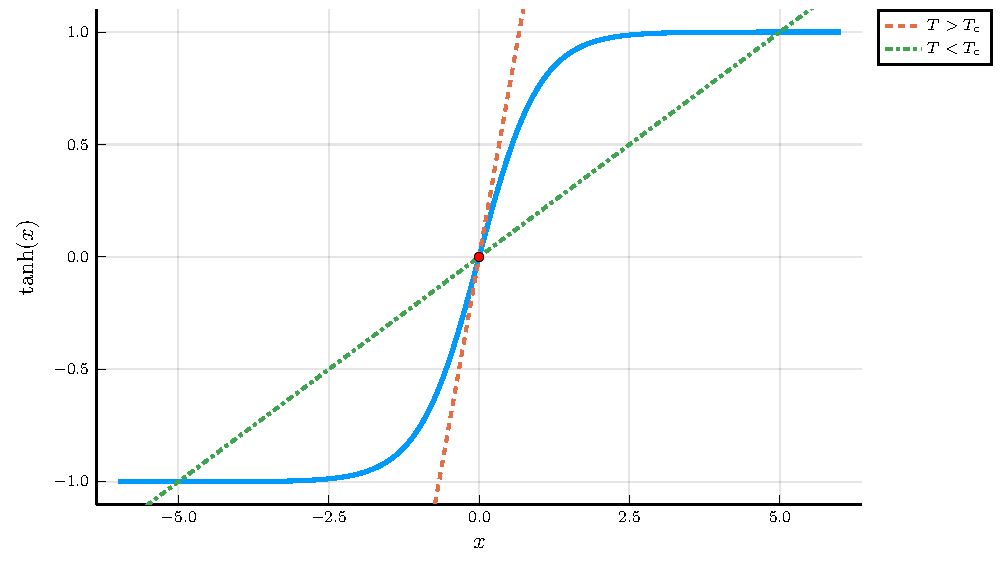
\includegraphics[scale=0.7]{codes/tanhx.pdf}
    \caption{Graphical analysis of the transcendental equation}
    \label{transcend}
\end{figure}
\noindent
In Fig.\ref{transcend}, we have plotted $\tanh(x)$ and two straight lines, with $T>Tc$ and $T<T_c$. For $T>Tc$, we see that the line does not cut $\tanh(x)$ at any point other than $x=0$. However, for $T<T_c$, we see that two solutions exist, other than the trivial solution $x=0$. As $\tanh(-x) = -\tanh(x)$, if one of the solution is $x=+x_0$, then the other solution is $x=-x_0$. A solution of $x$ corresponds to a solution of $\avg{\sigma}$. Thus, 
\begin{itemize}
    \item $T>T_c$ : $\avg{\sigma}=0$ is the only solution and there is no spontaneous magnetisation.
    \item $T<T_c$ : Apart from $\avg{\sigma}=0$, we have two other solutions $\avg{\sigma}=\pm m_0$.
\end{itemize}
The mean-field solution, which predicts a finite critical temperature, is clearly wrong for the 1D case, where we know that no phase transition occur at any finite temperature. In 1D, the fluctuations are too strong to throw away, since there are only two nearest neighbours to interact with.\\[0.2cm]
For the Ising model, two important things to note are \textit{dimensionality} and \text{lattice structure}. However, in the mean-field Hamiltonian, $\gamma$ (which is the only parameter depending on the topology of the lattice) cannot distinguish between these two factors. For example, for a cubic lattice in 3D, we have six nearest neighbours. Also, a triangular lattice in 2D has six nearest neighbours. Hence, these two lattices have the same $\gamma$, however, Ising dynamics in both the lattices are expected to be quite different.\\[0.2cm]
Mean-field analysis becomes exact if we increase the dimensionality of the lattice and also if we increase the range of interaction, that is, we include higher order neighbours also. This ensures that the interaction between the spins is indeed an \textit{effective interaction}.